\fancyhead[LE]{\fontsize{8.5pt}{10pt}\selectfont\textbf{\textsf{\thepage}}\quad \textbf{\textsf{CHƯƠNG 1}}\quad \textsf{Các hàm số và Mô hình}}
\fancyhead[RO]{\fontsize{8.5pt}{10pt}\selectfont\textsf{MỤC 1.1}\quad \textbf{\textsf{\thepage}}}

\noindent
\begin{minipage}[t]{0.265\textwidth}
    \fontsize{8pt}{10pt}\selectfont
    \vspace*{1.8cm}
    \begin{center}
        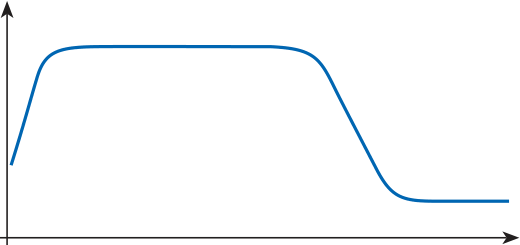
\includegraphics[width=0.92\linewidth]{images/p0047_fig11.png}\\[4pt]
        \textbf{\textsf{HÌNH 11}}
    \end{center}

    \vspace{4.0cm}
    \begin{center}
        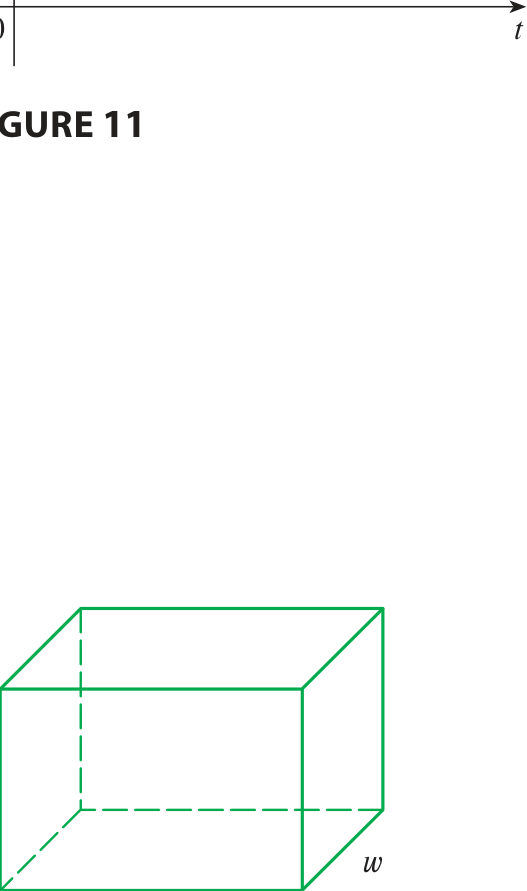
\includegraphics[width=0.92\linewidth]{images/p0047_fig12.png}\\[4pt]
        \textbf{\textsf{HÌNH 12}}
    \end{center}

    \vspace{1.0cm}
    \noindent
    \colorbox{purple!10}{%
        \begin{minipage}{0.96\linewidth}
            \vspace{3pt}
            \textbf{\colorbox{purple!80!black}{\color{white}\fontsize{7pt}{8pt}\selectfont\textsf{PS}}}\;%
            \fontsize{7.5pt}{9.5pt}\selectfont
            Khi thiết lập các hàm ứng dụng như trong Ví dụ 5, việc ôn lại các nguyên tắc giải quyết vấn đề ở cuối chương này có thể rất hữu ích, đặc biệt là \textit{Bước 1: Hiểu bài toán}.
            \vspace{3pt}
        \end{minipage}%
    }
\end{minipage}%
\hfill
\begin{minipage}[t]{0.708\textwidth}
    \fontsize{9.3pt}{13.2pt}\selectfont
    biết—biên độ và dạng sóng—đều có thể nhận thấy dễ dàng từ đồ thị. (Điều tương tự cũng đúng đối với các dạng sóng quan sát được trên điện tâm đồ của bệnh nhân tim và máy phát hiện nói dối.)

    Trong ví dụ tiếp theo, chúng ta phác họa đồ thị của một hàm số được xác định bằng lời văn.

    \vspace{0.25cm}
    \noindent
    \textbf{\textsf{\color{stewartcyan}VÍ DỤ 4}}\quad Khi bạn mở một vòi nước nóng được nối với bình nước nóng, nhiệt độ $T$ của nước phụ thuộc vào thời gian nước đã chảy. Hãy vẽ một đồ thị phác thảo của $T$ theo biến thời gian $t$ đã trôi qua kể từ khi vòi được mở.

    \vspace{0.15cm}
    \noindent
    \textbf{\textsf{\color{stewartcyan}LỜI GIẢI}}\quad Nhiệt độ ban đầu của nước chảy ra gần với nhiệt độ phòng vì lượng nước này nằm sẵn trong đường ống. Khi nước từ bình nước nóng bắt đầu chảy ra khỏi vòi, $T$ tăng lên nhanh chóng. Trong giai đoạn tiếp theo, $T$ không đổi ở mức nhiệt độ của nước nóng trong bình. Khi bình nước nóng cạn, $T$ giảm xuống nhiệt độ của nguồn nước cấp. Điều này cho phép chúng ta phác họa sơ bộ đồ thị của $T$ theo biến $t$ như được chỉ ra trong Hình 11. \hfill{\color{stewartcyan}$\blacksquare$}

    \vspace{0.3cm}
    Trong ví dụ sau, chúng ta bắt đầu với một mô tả bằng lời về một hàm số trong một tình huống vật lý và thu được một công thức đại số tường minh. Khả năng làm được điều này là một kỹ năng hữu ích trong việc giải các bài toán giải tích đòi hỏi tìm giá trị lớn nhất hoặc nhỏ nhất của các đại lượng.

    \vspace{0.25cm}
    \noindent
    \textbf{\textsf{\color{stewartcyan}VÍ DỤ 5}}\quad Một thùng chứa hình hộp chữ nhật không nắp có thể tích là $10\text{ m}^3$. Chiều dài của đáy gấp đôi chiều rộng của nó. Vật liệu làm đáy có giá $\$10$ mỗi mét vuông; vật liệu làm các mặt bên có giá $\$6$ mỗi mét vuông. Hãy biểu diễn chi phí vật liệu như một hàm số của chiều rộng đáy.

    \vspace{0.15cm}
    \noindent
    \textbf{\textsf{\color{stewartcyan}LỜI GIẢI}}\quad Ta vẽ sơ đồ như trong Hình 12 và đưa vào các ký hiệu bằng cách gọi $w$ và $2w$ lần lượt là chiều rộng và chiều dài của đáy, còn $h$ là chiều cao.
    
    Diện tích đáy là $(2w)w = 2w^2$, do đó chi phí (tính bằng đô la) của vật liệu làm đáy là $10(2w^2)$. Hai mặt bên có diện tích là $wh$ và hai mặt bên còn lại có diện tích là $2wh$, vì vậy chi phí vật liệu cho các mặt bên là $6[2(wh) + 2(2wh)]$. Do đó, tổng chi phí là
    \[
    C = 10(2w^2) + 6[2(wh) + 2(2wh)] = 20w^2 + 36wh
    \]
    Để biểu diễn $C$ chỉ theo biến $w$, chúng ta cần triệt tiêu $h$ và ta làm điều đó bằng cách sử dụng dữ kiện thể tích là $10\text{ m}^3$. Vì vậy
    \[
    w(2w)h = 10
    \]
    suy ra
    \[
    h = \frac{10}{2w^2} = \frac{5}{w^2}
    \]
    Thay biểu thức này vào công thức của $C$, ta được
    \[
    C = 20w^2 + 36w\left(\frac{5}{w^2}\right) = 20w^2 + \frac{180}{w}
    \]
    Do đó, phương trình
    \[
    C(w) = 20w^2 + \frac{180}{w}\qquad w > 0
    \]
    biểu diễn $C$ như một hàm số của $w$. \hfill{\color{stewartcyan}$\blacksquare$}

    \vspace{0.3cm}
    Trong ví dụ tiếp theo, chúng ta tìm tập xác định của một hàm số được xác định bằng biểu thức đại số. Nếu một hàm số được cho bởi một công thức và tập xác định không được nêu rõ, chúng ta sử dụng
\end{minipage}